\documentclass[12pt]{article}
\usepackage{graphicx}
\usepackage{amsmath}
\usepackage{hyperref}
\usepackage{caption}
\usepackage{float}
\usepackage{titlesec}
\usepackage[margin=1in]{geometry}
\usepackage[toc,page]{appendix}
\usepackage{geometry}
\usepackage{amsmath}
\usepackage{booktabs}
\usepackage{graphicx}
\usepackage{xcolor}
\usepackage{hyperref}
\usepackage{tabularx}
\usepackage{multirow}
\usepackage{subcaption}

\titleformat{\section}{\normalfont\Large\bfseries}{\thesection}{1em}{}
\titleformat{\subsection}{\normalfont\large\bfseries}{\thesubsection}{1em}{}

\title{NoMaD: \textbf{N}avigati\textbf{o}n with Goal-\textbf{Ma}sked \textbf{D}iffusion}
\author{Sehaj Ganjoo, Shobhnik Kriplani, \\ Abhishek Kumar Jha, Namashivayaa V \\ \texttt{Btech Mathematics and Computing} \\ Indian Institute of Science}
\date{\today}

\begin{document}
\maketitle

\begin{abstract}
This report presents our work on implementing and analyzing the training and perception components of a visual navigation system based on diffusion policies, as adapted from the NOMAD (Navigation with Goal Masked Diffusion) framework. 
Our approach combines a visual perception backbone based on EfficientNet and Transformer, with a trajectory diffusion model for motion planning to support both goal-directed and exploratory navigation. We trained our model on the SACSon,RECON and go\_stanford dataset, which features diverse real-world trajectories across various environments and robot platforms. 
We leverage a conditional diffusion model to generate multimodal waypoint predictions, enabling the agent to reason about complex, uncertain navigation scenarios. Our contributions include a detailed breakdown of the model architecture, training methodology, and evaluation metrics—particularly focusing on waypoint alignment through cosine similarity. 
We have left out the deployment aspects.
\end{abstract}

\section{Introduction}
Robotic learning for navigation in unfamiliar environments requires the ability to perform both task-oriented navigation (i.e., reaching a known goal) and task-agnostic exploration (i.e., searching for a goal in a novel environment). Traditionally, these functionalities are tackled by separate systems — for example, using subgoal proposals, explicit planning modules, or distinct navigation strategies for exploration and goal-reaching.

\subsection*{What is NoMaD?}
NoMaD is a transformer-based diffusion policy designed for long-horizon, memory-based navigation, that can:
\begin{itemize}
    \item Explore unknown places on its own (goal-agnostic behavior).
    \item Go to a specific place or object when given a goal image (goal-directed behavior).
\end{itemize}
Our project involves implementing the NoMaD Policy adapting its Transformer-based architecture and conditional diffusion decoder
to learn from a rich, multimodal dataset (SACSoN,SCAND,go\_stanford,RECON) composed of real-world trajectories.
Unlike traditional latent-variable models or methods that rely on separate generative components for subgoal planning, the unified diffusion policy exhibits superior generalization and robustness in unseen environments, while maintaining a compact model size.
In this report, we focus on the perception and training components of this policy, emphasizing how a strong visual encoder combined with a diffusion-based decoder leads to improved alignment of predicted and ground-truth waypoints. We analyze the training dynamics, present key quantitative metrics such as cosine similarity and distance loss, and highlight the model's ability to generalize across diverse scenarios.

\section{Methodology}
The NoMaD (Navigation with Goal-Masked Diffusion) framework introduces a unified visual navigation policy capable of both goal-conditioned navigation and open-ended exploration within a single architecture. Building on the Visual Navigation Transformer (ViNT) \cite{vint_paper} and diffusion-based policy learning (see Appendix \ref{app:preliminaries}), NoMaD extends these approaches with two key innovations: (1) attention-based goal masking for flexible behavior switching, and (2) a diffusion decoder for multimodal waypoint prediction.
\subsection*{Architecture Overview}
\label{subsec:architecture}
Figure \ref{fig:nomad_architecture} illustrates the NoMaD architecture, which consists of three main components:

\begin{figure}[H]
    \centering
    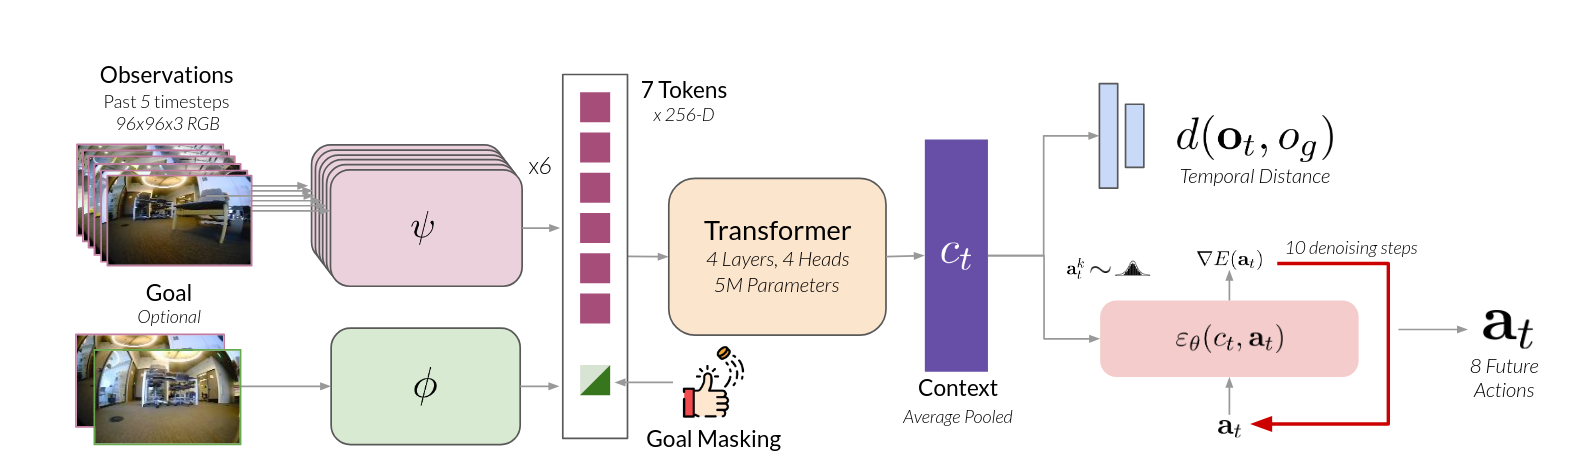
\includegraphics[width=0.85\textwidth]{nomad_diagram.png}
    \caption{NoMaD architecture. The visual encoder processes RGB observations, the transformer maintains temporal context, and the diffusion decoder generates waypoint predictions. Goal masking occurs in the attention layers of the context encoder.}
    \label{fig:nomad_architecture}
\end{figure}

\begin{itemize}
    \item \textbf{Visual Encoder}: Processes RGB observations $o_t$ using an EfficientNet-B0 backbone to extract feature embeddings.
    \item \textbf{Context Encoder}: Transformer-based module that maintains temporal context and handles goal conditioning
    \item \textbf{Diffusion Decoder}: Generates multimodal waypoint predictions through iterative denoising
\end{itemize}

\subsection*{A. Attention based Goal Masking}
\label{subsec:goal_masking}
To seamlessly switch between goal-directed behavior and exploration, we set a binary goal mask m in NoMaD.
The model builds on the ViNT (Visual Navigation Transformer) framework, by modifying the the computation of the observation context vector $c_t$ as follows:\\
\[
c_t = f(\psi(o_i), \phi(o_t, o_g), m)
\]
where:
\begin{itemize}
    \item $\psi(o_i)$: Encodes the current observation.
    \item $\phi(o_t, o_g)$: Encodes the time-step and goal image.
    \item $m$: A binary mask that determines whether to attend to the goal image or not.
\end{itemize}
\begin{itemize}
    \item When $m = 0$, the policy \textbf{attends to the goal image} $o_g$ to perform goal-conditioned navigation.
    \item When $m = 1$, the goal pathway is \textbf{masked out}, resulting in undirected exploration. Masking is applied in the attention layers, so goal embeddings are ignored if m=1.
\end{itemize}
During training, the goal mask $m$ is sampled from a Bernoulli distribution with probability $p_m = 0.5$, ensuring equal exposure to both behaviors. \\
At test time, $m$ is explicitly set based on the task: $m = 0$ for goal-reaching, and $m = 1$ for exploration.

\subsection*{B. Diffusion Policy}
Refer to Appendix for more on Diffusion policies.\\
In general, diffusion models are generative models that work by gradually adding noise to data (a forward process), and then learning to remove that noise (a reverse denoising process) to generate realistic samples.\\
To model complex, multimodal action distributions, especially in unstructured or ambiguous environments, NoMaD employs a \textbf{diffusion model} to approximate the conditional distribution of the next action as $p(a_t | c_t)$. \\
The denoising process is as follows:\\
1. \textbf{Forward Process:} Start with a real action $a^{0}_t$ from the dataset and add gaussian noise over multiple steps (K). 
\begin{center}
    $a^{k}_t = \sqrt{\alpha_k} a^{k-1}_t + (\sqrt{1 - \alpha_k}) \epsilon$
\end{center}
where:\\
\begin{itemize}
    \item $\epsilon$ $\sim$ $\mathcal{N}$(0,I) is a random noise
    \item $\alpha_k$ is a noise scheduler (eg square cosine)
    \item By step K, the action is almost pure noise.
\end{itemize}
2. \textbf{Reverse Denoising(Learned Model):} starting from pure noise $a^{k}_t$ $\sim$ $\mathcal{N}(0,I)$, it denoises step by step to recover the final clean action $a^{0}_t$.\\
Each denoising step is :
\begin{center}
    \[a^{k-1}_t = \alpha(\alpha^{k}_t-\gamma_k.\epsilon_{\theta}(c_t, a^{k}_t,k)) + \mathcal{N}(0,\sigma^2.I)\]
\end{center}
Where:
\begin{itemize}
    \item Here, $\epsilon_\theta$ is the noise prediction network conditioned on the context $c_t$, which may or may not include the goal depending on $m$.
    \begin{itemize}
        \item It is a 1D conditional U-Net with 15 CNN layers.
        \item Input:the noisy action $a^{k}_t$, the context vector $c_t$, and the diffusion step k.
        \item the predicted noise vector $\hat{\epsilon}_k$,During training, it is compared to the true noise added earlier.
    \end{itemize}
    \item $\gamma, \alpha ,\sigma$ are scheduler constants.
\end{itemize}

\subsection*{C. Implementation Details}
\subsection{Environment Setup}
All experiments were conducted on a system equipped with an NVIDIA GeForce GTX 1660 SUPER GPU and a 12\textsuperscript{th} Gen Intel\textregistered~Core\texttrademark~i9-12900K (24-core) processor. \\
The code was implemented in Python 3.12.9 in a conda environment. All the packages and libraries used are listed in the requirements.txt file.\\
The codebase was adapted from an open-source repository, and experiment tracking was performed using \texttt{Weights \& Biases (WandB)} for logging loss curves, evaluation metrics, and hyperparameter sweeps.
\subsection{Data Pipeline}
We trained the NoMaD model using the \textbf{SACSoN} and parts of \textbf{RECON} dataset, which contains diverse real-world trajectories across various environments and robot platforms.
The SACSoN dataset was already processed and we it split into training and validation sets using 80-20 split ratio. The RECON dataset consisted of bag files, which needed to be preprocessed to extract RGB images, actions, and ground-truth waypoints.
\subsection{Training Procedure}
Training was done on a single NVIDIA GPU using a batch size of 32 for 10 epochs.\\
\textbf{Training Objective:}\\
We calculate the Mean Squares Error(MSE) between  the predicted and the actual noise.
For overall loss function, we add the MSE temporal distance loss to the objective function.
\begin{center}
    \[ 
    \mathcal{L}_{NoMaD}(\phi,\psi,f,\theta,f_d) = MSE(\epsilon^{k}, \epsilon_{\theta}(c_t, a^{0}_t + \epsilon^{k},k)) + \lambda .MSE(d(o_t, o_g), f_{d}(c_t))
    \]
 \end{center}
 where:\\
 \begin{itemize}
     \item $\psi$,\ $\phi$ correspond to the visual encoders for the observation and goal images.
     \item $f$ corresponds to the transformer layers,
     \item $\theta$ corresponds to diffusion process parameters,
     \item $f_d$ corresponds to the temporal distance predictor.
 \end{itemize}

 \textbf{Training Configuration:}
 \begin{itemize}
     \item The weighting factor $\lambda$ for the auxiliary distance loss was set to $10^{-4}$.
     \item The model was trained using the \textbf{AdamW} optimizer with a learning rate of $1\text{e}^{-4}$ and a weight decay of $1\text{e}^{-2}$.
     \item We applied \textbf{cosine annealing} to decay the learning rate over time.
     \item We used \textbf{goal masking} with probability $p_m = 0.5$, encouraging the model to generalize across goal-visible and goal-agnostic contexts.
     \item The diffusion process used a \textbf{square cosine schedule} with $K = 10$ denoising steps.
     \item The ViNT observation encoder was an EfficientNet-B0, mapping $96 \times 96$ RGB images into a 256-dimensional latent embedding.
     \item The transformer used for context encoding had 4 layers and 4 attention heads.
     \item Training checkpoints and EMA snapshots were saved at the end of each epoch for model tracking and potential evaluation.
     \item Training and validation loss curves were logged using \texttt{Wandb} for detailed inspection.
\end{itemize}
\subsection{Evaluation}
We evaluate the model in two modes:\\ 
(i) \textbf{Unconditional (UC)}, where the policy predicts future waypoints based only on the observation history; and \\
(ii) \textbf{Goal-Conditioned (GC)}, where it also receives a goal image to guide planning. This distinction allows us to measure both general scene understanding and goal-directed behavior.

Evaluation was performed on the validation set using the following metrics:
\begin{itemize}
    \item distance loss
    \item diffusion loss
    \item cosine similarity
    \item action loss
\end{itemize}
\section{Experiments}
\subsection*{Goal-Conditioned (GC) Evaluation}
We set the goal mask $m = 0$ to evaluate the model's performance in goal-directed navigation.\\
\noindent \textbf{Distance Loss:}\\
\begin{figure}[H]
    \centering
    \begin{subfigure}[b]{0.48\textwidth}
        \centering
        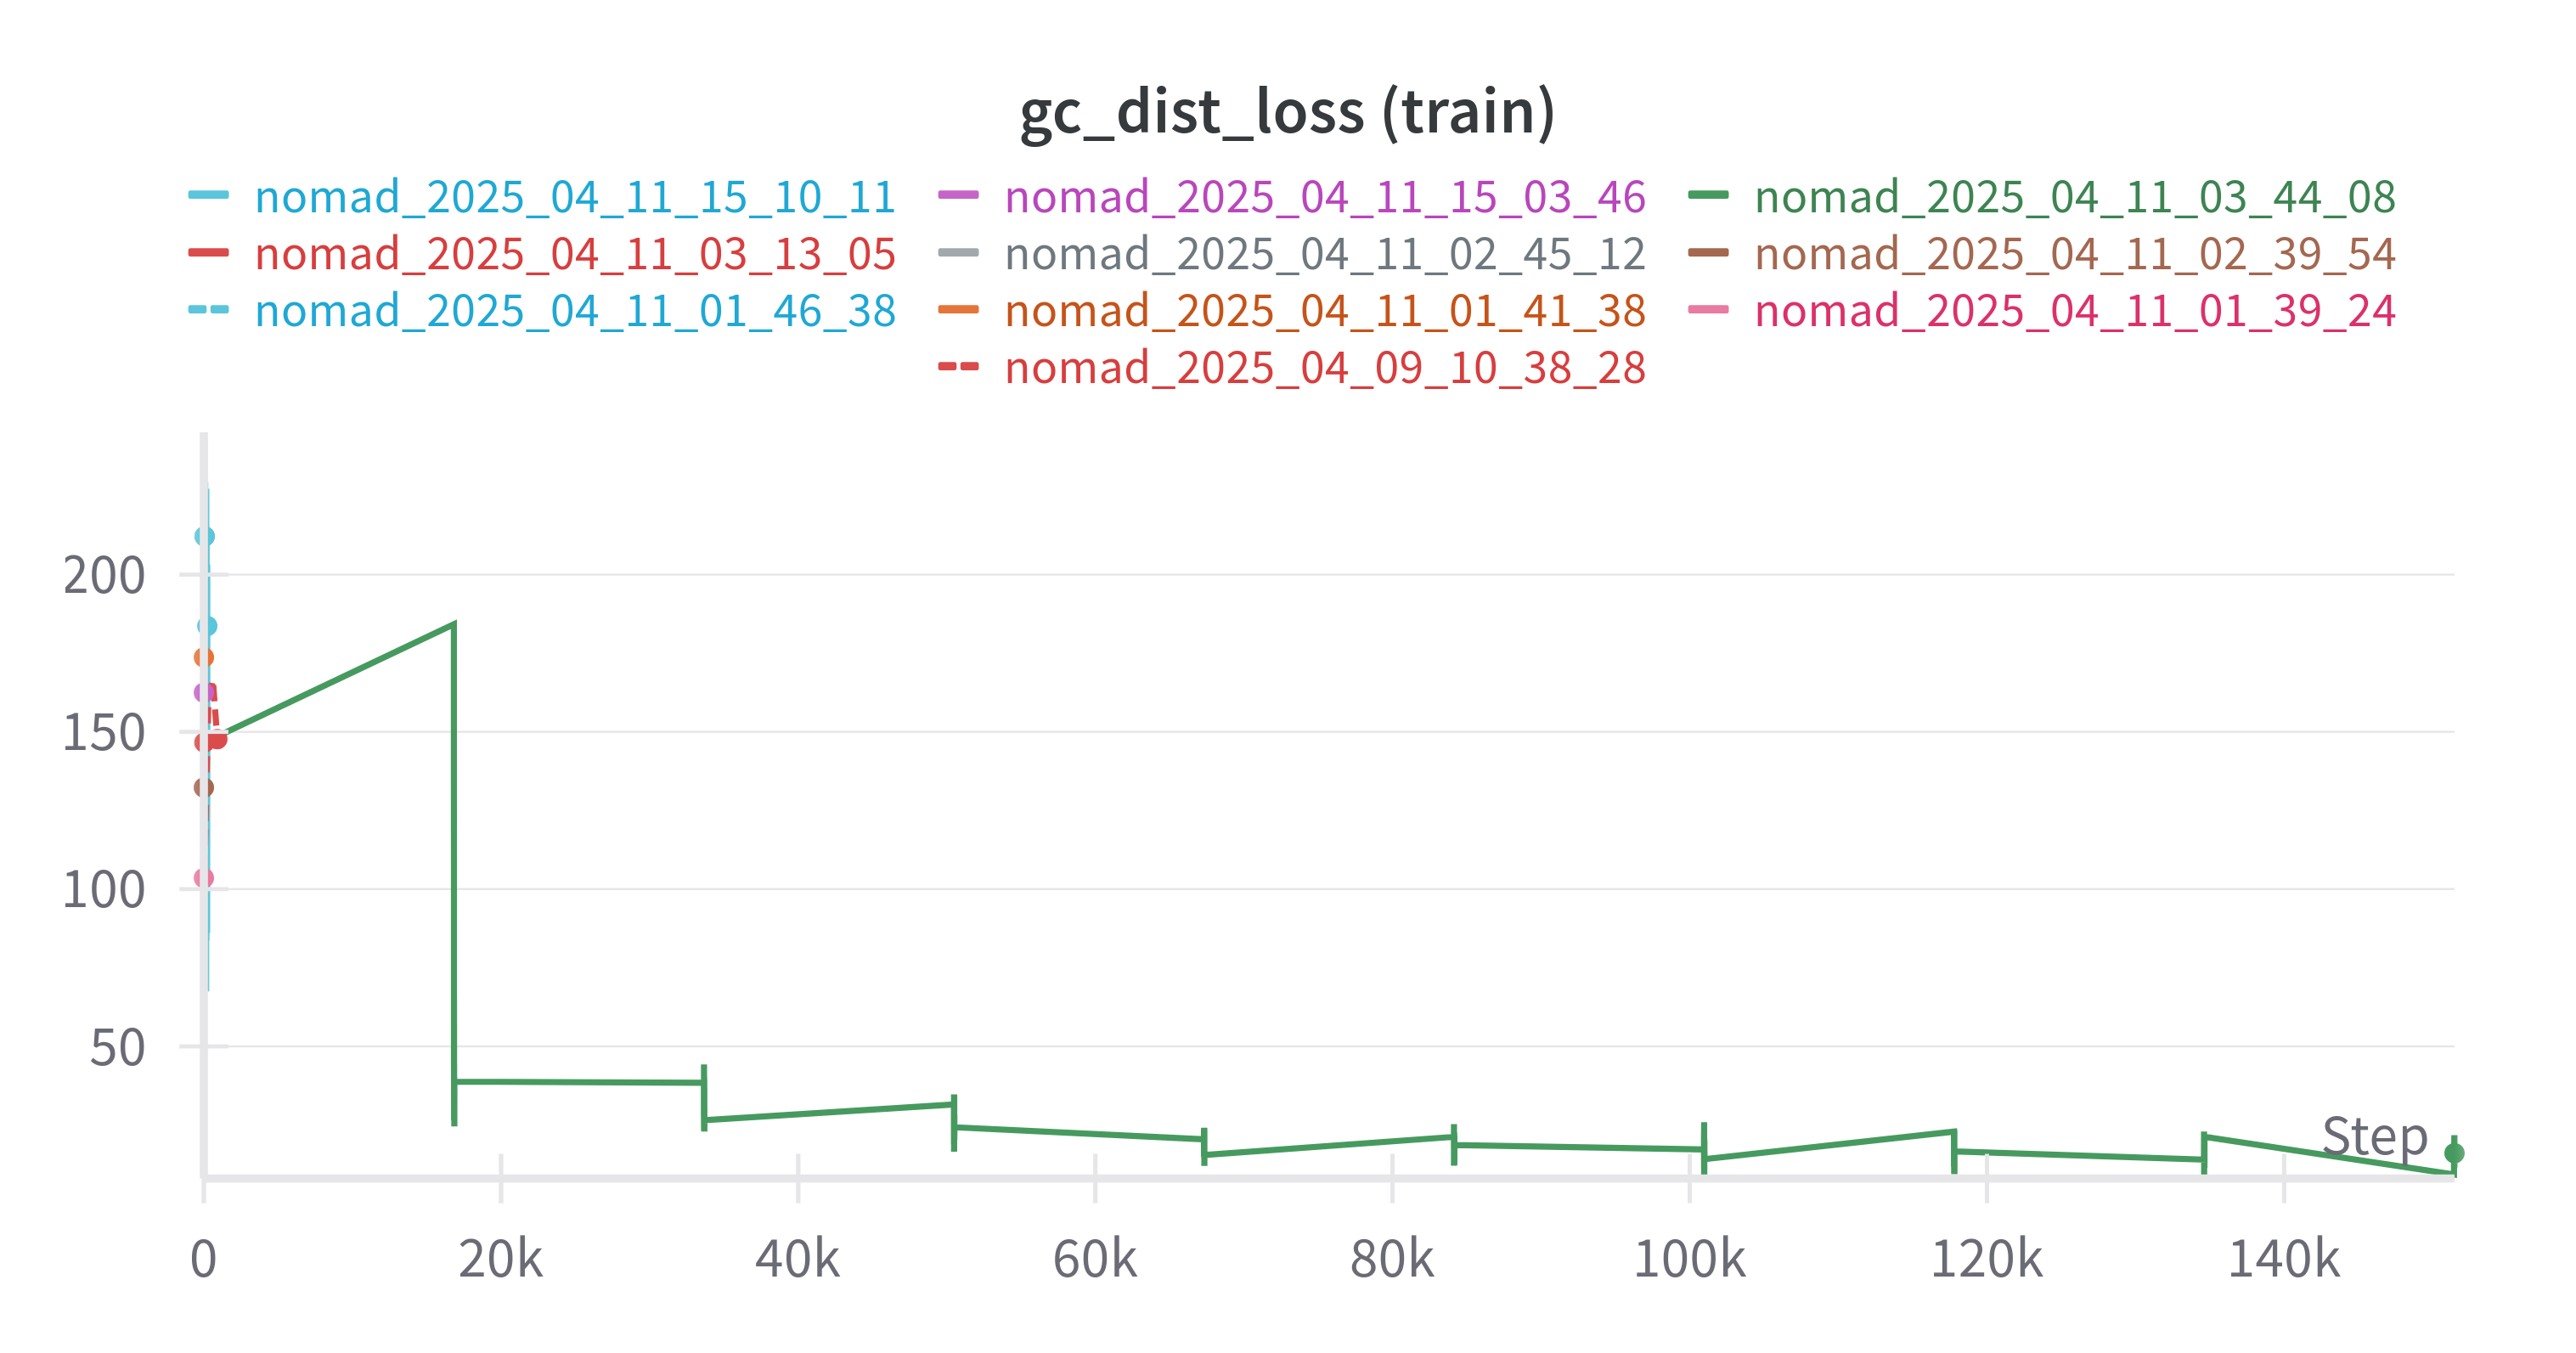
\includegraphics[width=\textwidth]{images/gc_distloss_nomad.png}
        \caption{Distance Loss on Training Set}
        \label{fig:gc_dist_loss_train}
    \end{subfigure}
    \hfill
    \begin{subfigure}[b]{0.48\textwidth}
        \centering
        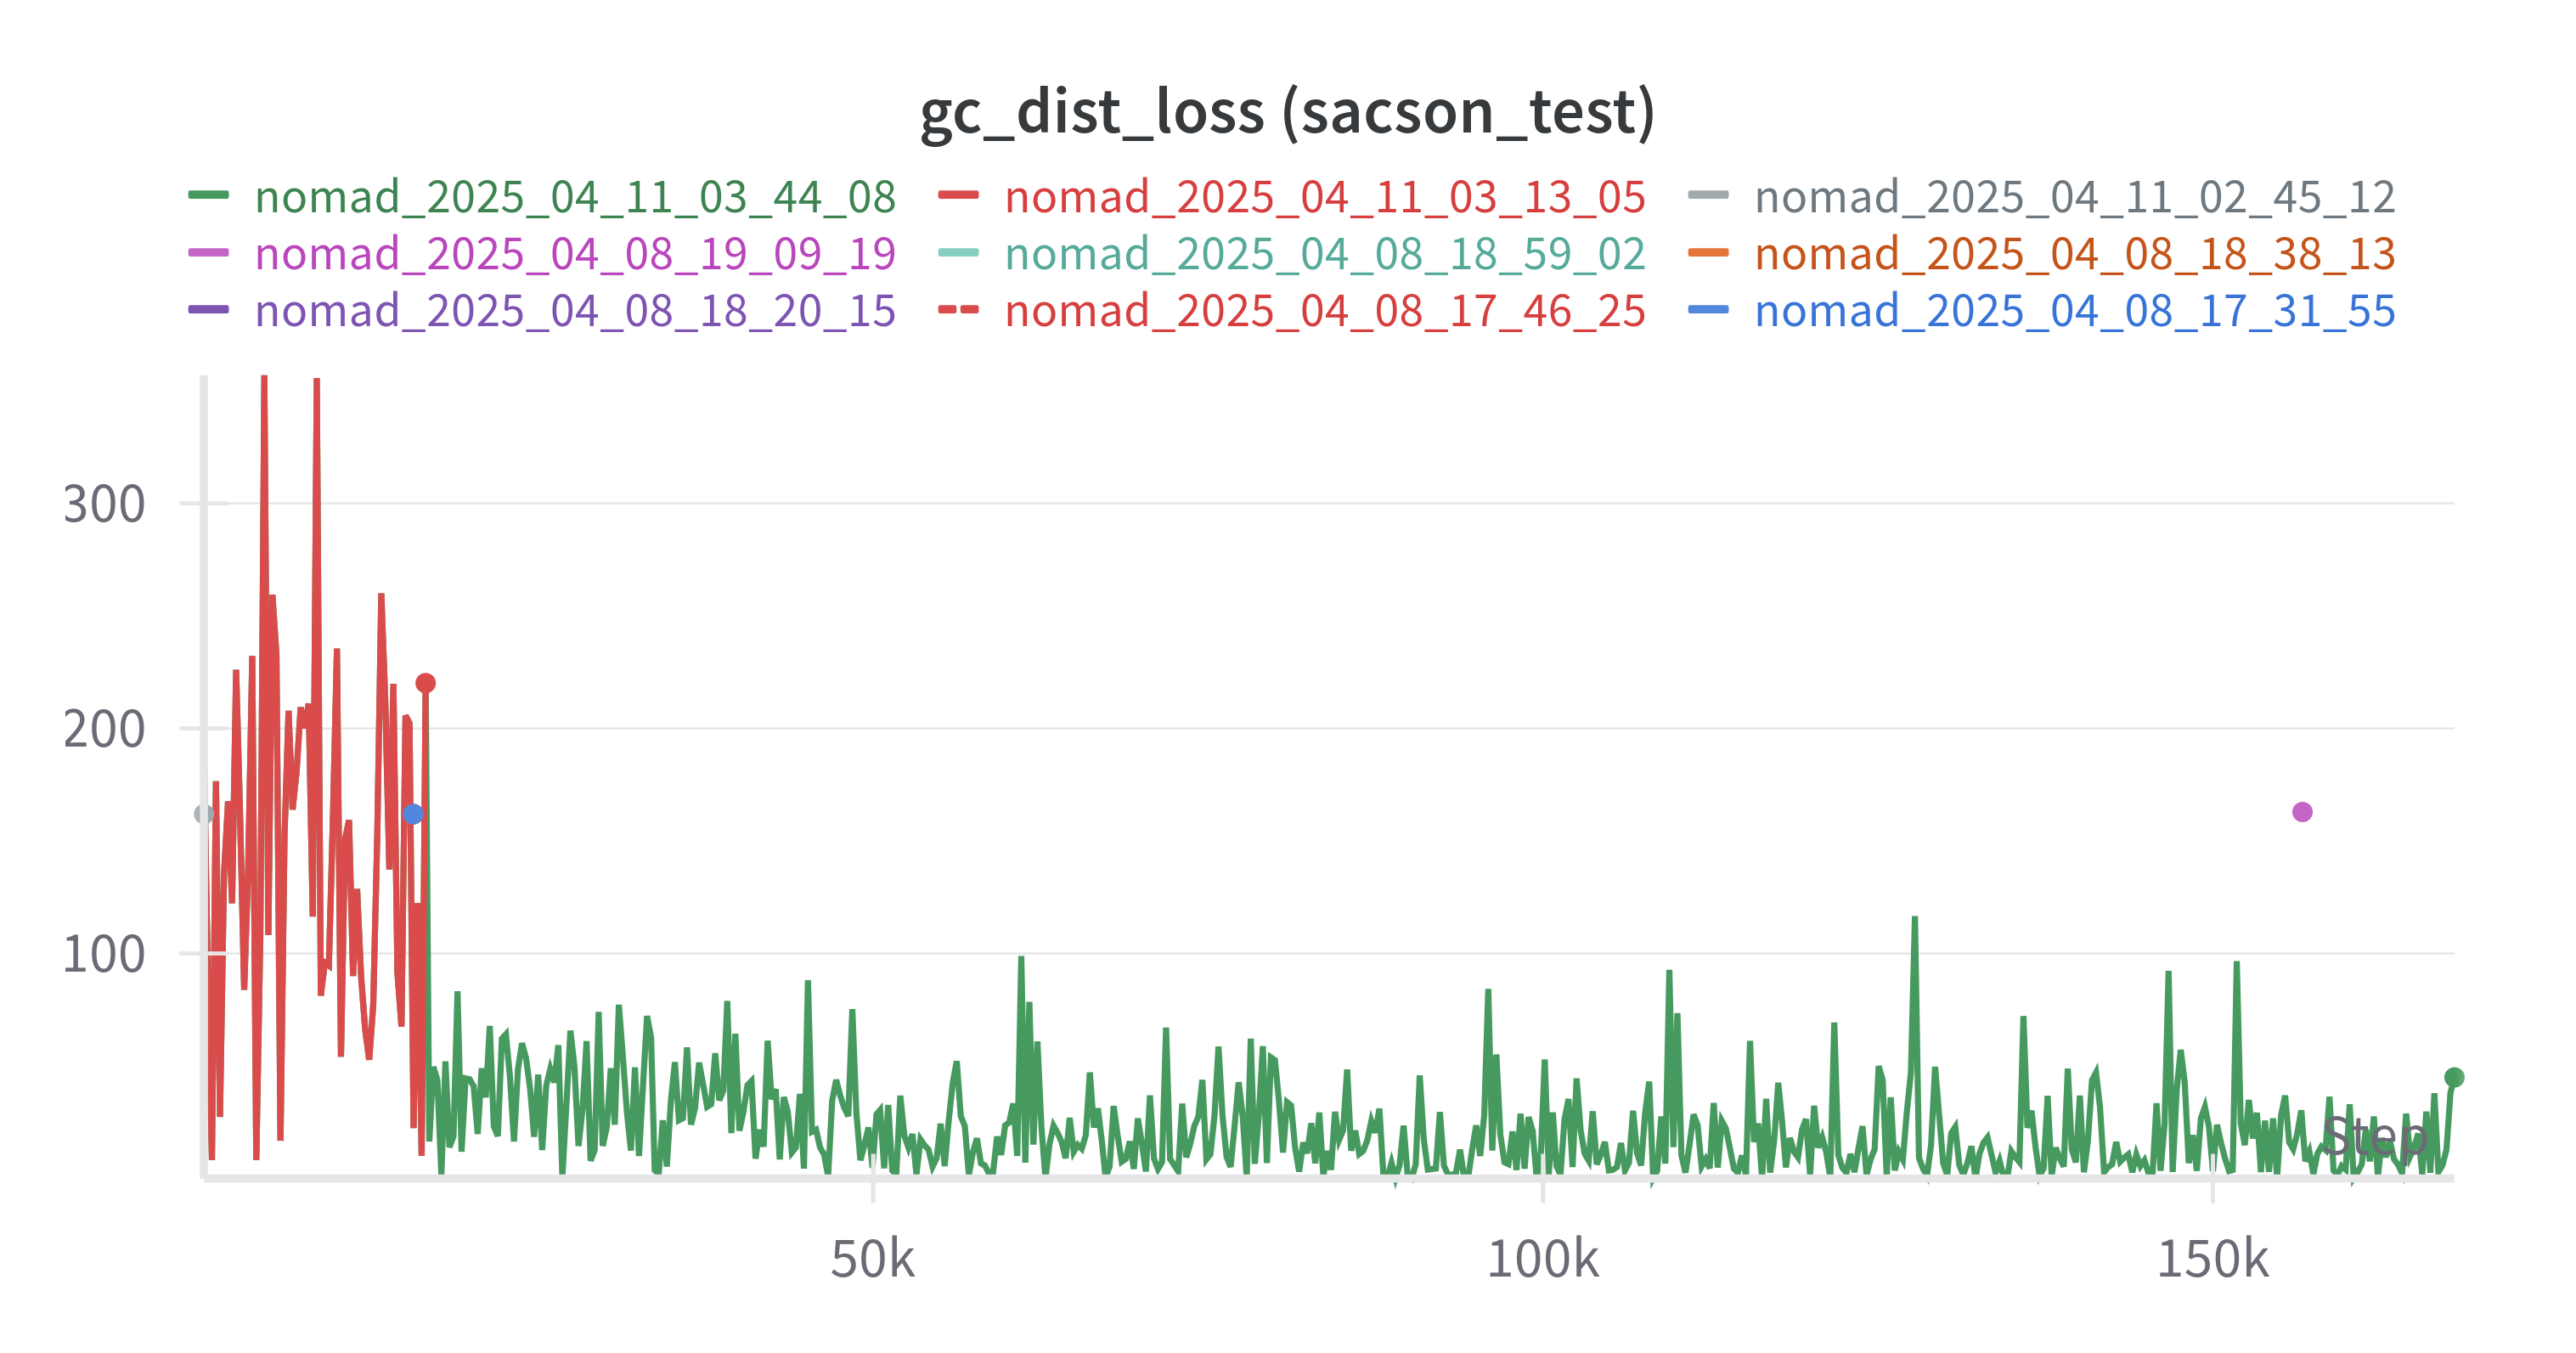
\includegraphics[width=\textwidth]{images/gc_dist_loss_test.png}
        \caption{Distance Loss on Validation Set}
        \label{fig:gc_dist_loss_val}
    \end{subfigure}
    \caption{Distance loss comparison between training and validation sets under goal-conditioned evaluation.}
\end{figure}






\subsection*{Comparison with ViNT}
To establish a baseline, we trained the original ViNT architecture using the same dataset and training hyperparameters as used for NoMaD.\\
We used the same EfficientNet-B0 encoder and transformer architecture, but without the diffusion decoder.\\
We evaluated both models under identical conditions on the validation set, using metrics such as Mean Squared Error (MSE) for actions and cosine similarity between predicted and ground-truth waypoints.\\
Interestingly, we observed that in the \textbf{goal-conditioned (GC)} setting, both ViNT and NoMaD achieved comparable performance across key metrics. This suggests that the introduction of a diffusion-based decoder in NoMaD does not degrade performance in goal-directed planning tasks. Instead, it provides a more expressive generative mechanism while maintaining task performance.\\
This supports the hypothesis that \textbf{diffusion-based modeling can match deterministic approaches in accuracy while offering better generative flexibility}, particularly for multi-modal or long-horizon planning scenarios.\\



\subsection{Training Metrics}
\begin{itemize}
\item Final training loss: \textasciitilde1.11
\item Cosine similarity: \textasciitilde0.47 (multi-action waypoints)
\item Distance loss: \textasciitilde128
\end{itemize}

\subsection{Observations}
Loss plateaued after around 5,000 batches. Training logs show improvement in cosine similarity and reduction in loss. Action losses remained stable across UC and GC branches.

\section{Challenges and Debugging}


\section{Conclusion and Future Work}
We successfully trained the NOMAD policy and analyzed the perception module. Future work could involve domain randomization, hyperparameter tuning, and evaluating transfer to real-world or simulated environments.

\section*{References}
\begin{enumerate}
\item H. Janner et al., "NOMAD: Planning with Diffusion for Visual Navigation," 2022.
\item Diffusion Policy GitHub Repository: \url{https://github.com/wayveai/diffusion-policy}
\end{enumerate}

\newpage
\begin{appendices}
\section{Related Work and \\ Contextual Foundations of NoMaD}
Exploration in unfamiliar enviroments is approached as the problem of efficient mapping, typically formulated around information maximization to guide the robot toward unexplored regions.\\
We factorize the classical exploration problem into two categories:\\
\begin{itemize}
    \item Local exploration strategies that rely on current observations. Objective is to learn control policies that can take diverse,short-horizon actions
    \item Global exploration strategies that utilize a map of the environment. Basically a high-level planner based on a topological graph that uses the policy for long-horizon goal-seeking
\end{itemize}
Robots exploring a new area are essentially trying to map it efficiently—this means covering as much area as possible, ideally without wasting time.\\
However, building detailed geometric maps, can be difficult without accurate depth perception. \\
Several prior approaches have investigated learning-based exploration policies. Some approaches use simulation data (training in virtual environments).\\
Others learn from real-world data directly. These models may use:\\
\begin{itemize}
    \item Intrinsic rewards: Encouraging the robot to explore new things.
    \item Semantic prediction: Going to interesting or informative places.
    \item Latent variable models: Abstract models of how actions affect the world.
\end{itemize}
Yet, policies trained in simulation frequently struggle to transfer to real-world environments. Even real-world-trained models can underperform in complex indoor and outdoor settings.\\
\bigskip
\noindent \textbf{Enter NoMaD : A New Method}\\ 
The work most closely related to NoMaD is ViNT (refer Appendix X for more details), which combines a goal-conditioned policy with a separate subgoal proposal module. The subgoal proposals are generated using an image diffusion model, condiitioned on robot's current view.\\
NoMaD improves on this by:
\begin{itemize}
    \item Not generating images.
    \item Directly predicting actions using diffusion models, which are typically used in image generation tasks but can model complex probabilities really well.
    \item This makes NoMaD more accurate and much lighter (needs 15x fewer parameters).
\end{itemize}
One of the core challenges in modeling robot exploration policies is the inherently multimodal nature of action sequences.\\
Observation-conditioned diffusion models  have emerged as powerful tools because they can learn complex action distributions without needing without needing explicit state prediction.\\
Nomad builds upon this adding \textbf{goal conditioning} to diffusion-based action generation, meaning it is capable of both:
\begin{itemize}
    \item Goal-directed exploration
    \item Undirected exploration 
\end{itemize}

\section{Technical Preliminaries}
The primary objective is to develop a visual navigation policy, denoted by $\pi$, that enables a robot to navigate using only RGB images from its onboard camera. \\
The policy devised should operates as follows:
\begin{itemize} 
    \item It receives a sequence of past and current observations: $o_t := o_{t-P : t}$. 
    \item It predicts a distribution over future actions: $a_t := a_{t : t+H}$. 
    \item Optionally, it can also condition on a goal image $o_g$, representing the desired destination. 
\end{itemize}
Depending on whether a goal is provided, the policy behaves differently: 
\begin{itemize} 
    \item \textbf{Goal-directed navigation:} When a goal image $o_g$ is available, $\pi$ generates actions that guide the robot toward the goal. 
    \item \textbf{Exploratory behavior:} When no goal is given (as in pure exploration settings), $\pi$ must still generate safe and purposeful actions—avoiding obstacles and staying on traversable paths—while efficiently covering the environment. 
\end{itemize}
To handle long-horizon planning and complex environments, the system is further augmented with: 
\begin{itemize} 
    \item A topological memory graph $\mathcal{M}$, which maintains a structured map of past visual observations. 
    \item A high-level planner that leverages this memory to decide on intermediate goals and broader exploration strategies. 
\end{itemize}
\subsection*{Visual Goal-Conditioned Policies: ViNT as the Backbone}
NoMaD builds on the ViNT (Visual Navigation Transformer) architecture, a Transformer-based model tailored for goal-conditioned navigation.\\
\paragraph{Key Components of ViNT:} 
\begin{itemize} 
    \item \textbf{Visual Encoding:} Each observation is processed using an EfficientNet-B0 encoder to extract feature embeddings. 
    \item \textbf{Goal Fusion:} The current and goal image features are combined using a goal fusion encoder. 
    \item \textbf{Transformer Attention:} These fused features (tokens) are passed through a Transformer model to generate a context vector $c_t$. 
    \item \textbf{Predictions:} The context vector is used to predict: 
    \begin{itemize} 
        \item A distribution over future actions: $a_t = f_a(c_t)$. 
        \item An estimate of temporal distance to the goal: $d(o_t, o_g) = f_d(c_t)$. 
    \end{itemize} 
\end{itemize}
These outputs are learned via supervised training, where the model is shown expert trajectories and learns to imitate them.
\begin{quote}
    \textit{However, ViNT is inherently goal-conditioned—it cannot operate in the absence of a goal image, limiting its ability to explore autonomously.} 
\end{quote}
\subsection*{Extending to Long-Horizon Planning with Topological Memory}
To overcome this limitation, NoMaD incorporates a topological memory $\mathcal{M}$: 
\begin{itemize} 
    \item Nodes represent previously encountered visual observations. 
    \item Edges represent traversable paths, established using ViNT's predicted distances. 
\end{itemize}
This memory graph enables both: 
\begin{itemize} 
    \item \textbf{Subgoal Planning:} If a goal cannot be reached directly, the planner identifies a sequence of reachable subgoals via $\mathcal{M}$. 
    \item \textbf{Structured Exploration:} Even without a goal, $\mathcal{M}$ helps guide exploration toward promising, yet-unvisited areas. 
\end{itemize}
\subsection*{Frontier-Based Exploration with NoMaD}
To evaluate NoMaD's ability to generalize to new environments, the authors implement a frontier-based exploration strategy:
\begin{itemize} 
    \item \textbf{Frontier:} The boundary between explored and unexplored areas in the environment. 
    \item The high-level planner selects frontiers as subgoals, encouraging the robot to expand coverage. 
\end{itemize}
This builds on the ViKiNG framework, but replaces its prior policy with NoMaD, which supports both: 
\begin{itemize} 
    \item \textbf{Goal-seeking} behavior (when a goal image is provided), and 
    \item \textbf{Autonomous exploration} (when no goal is available). 
\end{itemize}
\section{Vision Transformer (ViT)}

\subsection*{1. Core Architecture}
ViT adapts the \textbf{Transformer} architecture, originally designed for NLP, to \textbf{image recognition} by treating images as sequences of patches.

\subsubsection*{(a) Patch Embedding}
An input image $\mathbf{X} \in \mathbf{R}^{H \times W \times C}$ is split into $N$ non-overlapping patches of size $P \times P$. Each patch is flattened into a 1D vector and linearly projected:

\[
\mathbf{z}_i = \mathbf{E} \mathbf{x}_i + \mathbf{b}
\]

where:
\begin{itemize}
    \item $\mathbf{x}_i \in \mathbf{R}^{P^2 \times C}$ is the flattened patch
    \item $\mathbf{E} \in \mathbf{R}^{D \times P^2 C}$ is the embedding matrix
    \item $D$ is the embedding dimension (e.g., 768)
\end{itemize}

For an image of size 224$\times$224 and patch size 16$\times$16:

\[
N = \left( \frac{224}{16} \right)^2 = 196 \text{ patches}
\]

\subsubsection*{(b) Class Token (CLS)}
A learnable classification token $\mathbf{z}_{cls} \in \mathbf{R}^D$ is prepended:

\[
\mathbf{Z} = [\mathbf{z}_{cls}; \mathbf{z}_1; \mathbf{z}_2; \dots; \mathbf{z}_N]
\]

\subsubsection*{(c) Positional Embeddings}
Learned positional embeddings are added to retain spatial information:

\[
\mathbf{Z} = \mathbf{Z} + \mathbf{E}_{pos}, \quad \mathbf{E}_{pos} \in \mathbf{R}^{(N+1) \times D}
\]

\subsection*{2. Transformer Encoder}
The ViT encoder consists of \textbf{L identical layers}, each containing:

\begin{itemize}
    \item Multi-Head Self-Attention (MHSA)
    \item Layer Normalization (LN)
    \item Feed-Forward Network (FFN)
    \item Residual Connections
\end{itemize}

\subsubsection*{(a) Multi-Head Self-Attention (MHSA)}
Input embeddings are split into $h$ heads (e.g., 12 heads for ViT-Base). For each head:

\[
\text{Attention}(\mathbf{Q}, \mathbf{K}, \mathbf{V}) = \text{softmax}\left( \frac{\mathbf{Q} \mathbf{K}^T}{\sqrt{d_k}} \right) \mathbf{V}
\]

where $d_k = D / h$.

\subsubsection*{(b) Feed-Forward Network (FFN)}
A 2-layer MLP with GELU activation:

\[
\text{FFN}(\mathbf{x}) = \mathbf{W}_2 \text{GELU}(\mathbf{W}_1 \mathbf{x} + \mathbf{b}_1) + \mathbf{b}_2
\]

where:
\begin{itemize}
    \item $\mathbf{W}_1 \in \mathbf{R}^{4D \times D}$
    \item $\mathbf{W}_2 \in \mathbf{R}^{D \times 4D}$
\end{itemize}

\subsubsection*{(c) Layer Normalization \& Residual Connections}
Each sub-layer is wrapped with:

\[
\mathbf{x}_{\text{out}} = \text{LayerNorm}(\mathbf{x} + \text{SubLayer}(\mathbf{x}))
\]

\subsection*{3. Training \& Fine-Tuning}
\begin{itemize}
    \item \textbf{Pre-training}: On large datasets (e.g., JFT-300M)
    \item \textbf{Fine-tuning}: Adapt to downstream tasks by replacing classification head
\end{itemize}

\section{EfficientNet}

\subsection*{1. Compound Scaling}
EfficientNet introduces \textbf{compound scaling}:

\[
d = \alpha^\phi, \quad w = \beta^\phi, \quad r = \gamma^\phi
\]

where:
\begin{itemize}
    \item $\phi$ is a scaling coefficient
    \item $\alpha, \beta, \gamma$ are constants ($\alpha = 1.2, \beta = 1.1, \gamma = 1.15$)
\end{itemize}

\textbf{Constraint}:
\[
\alpha \cdot \beta^2 \cdot \gamma^2 \approx 2
\]

\subsection*{2. MBConv Block}
The core building block consists of:
\begin{itemize}
    \item 1×1 Expansion Conv (expansion factor $t=6$)
    \item Depthwise Conv
    \item Squeeze-and-Excitation (SE) Block
    \item 1×1 Projection Conv
\end{itemize}

\subsubsection*{(a) Depthwise Separable Convolution}
\begin{itemize}
    \item \textbf{Depthwise Conv}:
    \[
    \mathbf{y}_{i,j,k} = \sum_{m,n} \mathbf{K}_{m,n,k} \mathbf{x}_{i+m, j+n, k}
    \]
    \item \textbf{Pointwise Conv}:
    \[
    \mathbf{z}_{i,j,l} = \sum_k \mathbf{W}_{k,l} \mathbf{y}_{i,j,k}
    \]
\end{itemize}

\subsubsection*{(b) Squeeze-and-Excitation (SE)}
\begin{itemize}
    \item \textbf{Squeeze}: Global average pooling $\rightarrow \mathbf{s} \in \mathbf{R}^C$
    \item \textbf{Excitation}:
    \[
    \mathbf{s}_{excite} = \sigma(\mathbf{W}_2 \text{ReLU}(\mathbf{W}_1 \mathbf{s}))
    \]
    \item \textbf{Rescale}:
    \[
    \mathbf{x}_{out} = \mathbf{s}_{excite} \odot \mathbf{x}
    \]
\end{itemize}

\subsection*{3. Neural Architecture Search (NAS)}
EfficientNet-B0 was discovered using:

\[
\text{maximize } \text{ACC}(m) \times \left[ \frac{\text{FLOPS}(m)}{T} \right]^w
\]

where:
\begin{itemize}
    \item $w = -0.07$
    \item $T = 400M$ (target FLOPS for B0)
\end{itemize}

\begin{thebibliography}{9}
\bibitem{vit} 
Dosovitskiy et al. 
\textit{An Image is Worth 16x16 Words: Transformers for Image Recognition at Scale}. 
2021. 
\href{https://arxiv.org/abs/2010.11929}{arXiv:2010.11929}

\bibitem{effnet} 
Tan \& Le. 
\textit{EfficientNet: Rethinking Model Scaling for Convolutional Neural Networks}. 
2019. 
\href{https://arxiv.org/abs/1905.11946}{arXiv:1905.11946}
\end{thebibliography}

\end{appendices}
\end{document}